% =====================================================================
% DRAFT 4 (24 Oct 2026), IEEE conference template (IEEEtran, conference)
%
% Every number is traced to docs/results/selective.json (generator 1.0,
% seed 7, commit a091d11), rendered as docs/results/selective.md. The
% plan and hypotheses are in docs/RESEARCH_PAPER_PLAN.md and
% docs/RESEARCH_GAP_ANALYSIS.md. Items still open are marked \todo{...}
% (red). Remove all \todo marks before submission.
%
% Figures are drawn with TikZ/pgfplots from the numbers in selective.json,
% so there are no image files to keep in sync.
%
% Compile:  pdflatex paper.tex && pdflatex paper.tex   (or: tectonic paper.tex)
%
% REFERENCES: see the comment above each \bibitem.
%   VERIFIED-GA = metadata verified on 16 Oct 2026 for the research gap
%                 analysis (Crossref / DataCite / arXiv API / publisher page).
%   VERIFIED-D1 = checked against a web source on 23 Oct 2026 for draft 1.
%   CARRIED     = copied from the project report; not re-verified.
%   Re-run the literature search within four weeks of submission
%   (RESEARCH_PAPER_PLAN.md 9.9).
% =====================================================================
\documentclass[conference]{IEEEtran}
\IEEEoverridecommandlockouts
\usepackage{cite}
\usepackage{amsmath,amssymb,amsfonts}
\usepackage{algorithmic}
\usepackage{graphicx}
\usepackage{subcaption}
\usepackage{textcomp}
\usepackage{xcolor}
\usepackage{url}
\usepackage{tikz}
\usetikzlibrary{positioning,arrows.meta,shapes.geometric}
\usepackage{pgfplots}
\pgfplotsset{compat=1.17}
\usepackage{fancyhdr}
\usepackage{hyperref}
\hypersetup{hidelinks}
\def\BibTeX{{\rm B\kern-.05em{\sc i\kern-.025em b}\kern-.08em
    T\kern-.1667em\lower.7ex\hbox{E}\kern-.125emX}}

% First-page conference header and copyright footer, as in the TEMSMET 2026
% papers. The ISBN/price line is the one used by the VEDA paper; take the
% exact line from the conference's camera-ready instructions, and delete
% this block for any other venue.
\fancypagestyle{firstpage}{%
  \fancyhf{}%
  \fancyhead[L]{\parbox[t]{\textwidth}{\raggedright\footnotesize
    International Conference on Technology, Engineering, Management for Societal
    Impact using Marketing, Entrepreneurship\\ and Talent (TEMSMET 2026)}}%
  \fancyfoot[L]{\footnotesize 979-8-3195-2359-4/26/\$31.00 \textcopyright2026 IEEE}%
  \renewcommand{\headrulewidth}{0pt}%
  \renewcommand{\footrulewidth}{0pt}%
}

\newcommand{\todo}[1]{\textbf{\textcolor{red}{[TODO: #1]}}}
\newcommand{\sysB}{\textsf{B0}}
\newcommand{\sysBtwo}{\textsf{B2}}
\newcommand{\sysBone}{\textsf{B1}}
\newcommand{\sysP}{\textsf{P}}
\newcommand{\sysFC}{\textsf{FC}}
\newcommand{\sysPdup}{\textsf{P+dup}}

\begin{document}

% No funding to declare, so no \thanks{} line.
\title{Measuring the Value of Enterprise Records in Risk-Controlled Invoice Automation}

\author{\IEEEauthorblockN{Anjali Dinesh Jayashree More}
\IEEEauthorblockA{\textit{Department of Computer Engineering} \\
\textit{Fr. C. Rodrigues Institute of Technology}\\
Navi Mumbai, Maharashtra, India \\
anjalidineshmore@gmail.com}
\and
\IEEEauthorblockN{Vaidehi Jagdeep Sankaye}
\IEEEauthorblockA{\textit{Department of Computer Engineering} \\
\textit{Fr. C. Rodrigues Institute of Technology}\\
Navi Mumbai, Maharashtra, India \\
vjsankaye@gmail.com}
\and
\IEEEauthorblockN{Niraj Ravindra Sawant}
\IEEEauthorblockA{\textit{Department of Computer Engineering} \\
\textit{Fr. C. Rodrigues Institute of Technology}\\
Navi Mumbai, Maharashtra, India \\
nirajsawant203@gmail.com}
\and
\IEEEauthorblockN{Anooj Vinayak Shete}
\IEEEauthorblockA{\textit{Department of Computer Engineering} \\
\textit{Fr. C. Rodrigues Institute of Technology}\\
Navi Mumbai, Maharashtra, India \\
anoojshete@gmail.com}
\and
\IEEEauthorblockN{Dr. Jyoti More}
\IEEEauthorblockA{\textit{Department of Computer Engineering} \\
\textit{Fr. C. Rodrigues Institute of Technology}\\
Navi Mumbai, Maharashtra, India \\
\todo{email or ORCID}}
}

\maketitle
\thispagestyle{firstpage}

% Template rule: no symbols, special characters, footnotes or math in the
% title or abstract, so percentages are spelled out here.
\begin{abstract}
Many procure-to-pay systems post an invoice without human review once its
extraction confidence passes a fixed threshold. The error rate such a threshold
lets through is seldom measured. It is also unclear whether checks against the
organization's own records (vendor master, open purchase orders, earlier
invoices) would let more invoices skip review at the same error rate. We study
both questions on a seeded synthetic procure-to-pay world of 100 vendors, 1,649
purchase orders and 3,000 invoices, of which 29.8 percent carry one injected
business error. Invoices are rendered as text PDFs or as scans of three quality
levels and read with the extraction code of a deployed platform. We compare the
platform's confidence rule, a rule that accepts when every record check passes,
and risk-controlled gates that pick their threshold with Learn-then-Test, using
document evidence alone or document and record evidence, over 20 vendor-disjoint
splits. The deployed rule accepts 41.2 percent of invoices, and 6.8 percent of
those are wrong. Record evidence improves ranking (AUROC rises from 0.724 to 0.947
with gradient boosting), but no pre-specified gate certifies more than 1.7
percent of invoices at error budgets of 1, 2 or 5 percent, so our pre-registered
hypothesis of a five-point coverage gain is not supported. Most errors among the
top-ranked invoices are resubmissions under a new invoice number, which the
production duplicate rule misses. A duplicate check that ignores the number,
defined after this diagnosis, certifies 12.1 and 35.4 percent of invoices at the
2 and 5 percent budgets. All data are synthetic and come from one generator, and
the post hoc result needs replication.
\end{abstract}

\begin{IEEEkeywords}
selective prediction, risk control, Learn-then-Test, invoice processing,
procure-to-pay, straight-through processing
\end{IEEEkeywords}

% ---------------------------------------------------------------------
\section{Introduction}\label{sec:intro}
An automated procure-to-pay (P2P) pipeline reads each incoming invoice, links it
to a vendor and a purchase order (PO), and then either posts it or sends it to a
person. Posting without review is a \emph{selective prediction} decision: the
system trades coverage, the share of documents handled automatically, against
the error rate among the documents it accepts \cite{elyaniv2010,geifman2017}.
Work on document extraction usually reports field accuracy on benchmarks such as
SROIE \cite{huang2019sroie}, or the results of layout-aware models such as
LayoutLMv3 \cite{huang2022layoutlmv3}. A posting gate is judged differently. What
counts is how many accepted invoices are wrong, and an invoice can be wrong even
when every field was read correctly: it may be a resubmission, carry changed bank
details, or bill more than was ordered.

Learn-then-Test (LTT) \cite{angelopoulos2025ltt} chooses a threshold so that the
error rate among accepted items stays below a target with high probability.
Recent work applies this kind of guarantee to straight-through processing of
financial documents \cite{jin2026plv,rombach2026}, but scores each document, and
usually each field, on what the document itself contains. Commercial P2P tools
do match invoices against vendor masters and POs \cite{rossum2026,sapariba2026},
with tolerances set by hand and no published error rates.

This paper starts from the review gate of a procurement platform we
built. It accepts an invoice when a weighted extraction
confidence is at least 0.8 and no review flag is raised. We ask four research
questions (RQs):
\begin{itemize}
\item \textbf{RQ1.} What error rate does this fixed rule admit on an invoice
stream that contains business errors?
\item \textbf{RQ2.} Does evidence from the organization's records let a
risk-controlled gate accept more invoices at the same error budget? Our
pre-registered hypothesis (H1) was a gain of at least 5 percentage points over a
document-only gate at an error budget of 2\%.
\item \textbf{RQ3.} Is it better to control risk for the whole document or to
combine one gate per field?
\item \textbf{RQ4.} How much of the ranking signal survives when the records
are out of date?
\end{itemize}

The contributions are empirical. We do not propose a new risk-control method or
a new extractor. (1)~We measure the error rate of the deployed rule, and of a
rule that trusts every record check, on a P2P benchmark with known ground truth.
(2)~We compare risk-controlled gates with and without record evidence over
vendor-disjoint splits, with an ablation per check and a stale-records test.
(3)~We explain why no pre-specified gate certifies a useful share, and report a
post hoc fix together with what it needs before it can be trusted.

Section~\ref{sec:related} reviews related work and Section~\ref{sec:problem}
states the problem. Section~\ref{sec:method} describes the gates and the
benchmark, Section~\ref{sec:setup} the protocol, and Section~\ref{sec:results}
the results. Limitations follow in Section~\ref{sec:limits}.

% ---------------------------------------------------------------------
\section{Related Work}\label{sec:related}
\subsection{Selective Prediction and Risk Control}
Selective classification lets a model abstain to lower its risk. El-Yaniv and
Wiener describe the resulting risk--coverage trade-off for noise-free
models \cite{elyaniv2010}, and Geifman and El-Yaniv build a selective classifier
on top of a trained network so that a chosen risk level holds with high
probability \cite{geifman2017}. LTT treats the choice of a low-dimensional
parameter, such as a threshold, as a multiple-testing problem and gives
finite-sample guarantees for any underlying model \cite{angelopoulos2025ltt};
conformal risk control does the same for the expected value of a monotone
loss \cite{angelopoulos2024crc}. In both, the guarantee holds whatever the
quality of the score. The coverage obtained does not: it depends on how well the
score separates correct from incorrect items, which is what RQ2 varies.

Learning to defer models the human who receives rejected
items \cite{madras2018,mozannar2020}. We treat review as a fixed, error-free
fallback and list this as a limitation. Raw confidence scores of neural networks
are often miscalibrated \cite{guo2017}, and the platform's field confidences are
hand-set constants, which is one reason to learn a probability model on labeled
data before thresholding it. LTT also assumes that calibration and deployment
data are exchangeable. Weighted conformal prediction relaxes this under
covariate shift when the likelihood ratio is known or can be
estimated \cite{tibshirani2019}; we do not apply it (Section~\ref{sec:limits}).

\subsection{Document Extraction and Its Benchmarks}
Layout-aware pretrained models read business documents
well \cite{huang2022layoutlmv3}, and optical character recognition (OCR) and
conversion engines such as PaddleOCR and Docling are widely used in
practice \cite{cui2025paddleocr,auer2024docling}. The benchmarks measure reading.
SROIE covers receipts \cite{huang2019sroie}; DocILE \cite{simsa2023docile} and
FATURA \cite{limam2023fatura} cover invoices. None of them ships the purchase
orders, vendor master or payment history an invoice belongs to, so none can say
whether posting it was right. Krieger \emph{et al.}\ show that extractors degrade
on rarely seen suppliers \cite{krieger2023}, which bears on gates evaluated on
unseen vendors.

\subsection{Confidence for Straight-Through Processing}
HYCEDIS scores extracted key--value pairs with a conformal predictor and an
anomaly detector \cite{nguyen2022hycedis}. Rombach and Mehdiyev build
entity-level conformal prediction sets for receipts and propose to accept
singletons \cite{rombach2026}. ConfBench measures how well the confidence of
vision--language models tracks extraction accuracy under document
degradation \cite{roy2026confbench}. The closest work is that of Jin
\emph{et al.}~\cite{jin2026plv}: they fuse perception, layout and validation
features with gradient boosting and set per-field thresholds with LTT on DocILE,
FATURA and VRDU. Their validators are document-internal (formats, checksums,
arithmetic, a second model), they report that these add little signal on
invoices, and their decisions are per field.

\subsection{Procurement Practice and the Gap}
Reviews of artificial intelligence in procurement find most deployments in the
P2P cycle \cite{guida2023,spreitzenbarth2024}, and three-way matching against
POs and receipts is standard in commercial tools \cite{rossum2026,sapariba2026}.
Table~\ref{tab:compare} sets these lines of work side by side. Within the
literature we searched, no study (i)~measures the error admitted by a
confidence-threshold gate on invoices with business errors, or (ii)~tests
whether evidence from enterprise records changes what a risk-controlled gate can
certify, at the level of the whole document. Practice already uses these checks
as hard rules, so the idea of matching is not new; what has not been measured is
its value inside a gate with an error guarantee.

\begin{table}[t]
\caption{Closest Work Compared with This Study}
\begin{center}
\setlength{\tabcolsep}{3pt}
\resizebox{\columnwidth}{!}{%
\begin{tabular}{|l|c|c|c|c|}
\hline
\textbf{Work} & \textbf{Error guarantee} & \textbf{Record evidence} & \textbf{Decision unit} & \textbf{Contribution measured} \\
\hline
Jin \emph{et al.} \cite{jin2026plv} & LTT & no & field & n/a \\
Rombach and Mehdiyev \cite{rombach2026} & conformal sets & no & entity & n/a \\
ConfBench \cite{roy2026confbench} & none & no & entity & n/a \\
Rossum \cite{rossum2026} & none published & yes (rules) & field & no \\
SAP Ariba \cite{sapariba2026} & none published & yes (rules) & invoice & no \\
This study & LTT & yes & invoice & yes (ablation) \\
\hline
\multicolumn{5}{l}{\footnotesize Based on the published text and documentation
reviewed in October 2026.}
\end{tabular}}
\label{tab:compare}
\end{center}
\end{table}

% ---------------------------------------------------------------------
\section{Problem Formulation}\label{sec:problem}
Each invoice $i$ has document evidence $D_i$ (extracted fields, field
confidences, text quality, classification confidence, internal consistency
checks), record evidence $E_i$ (results of checks against the vendor master,
open POs and earlier invoices), and a label $Y_i\in\{0,1\}$. We set $Y_i=1$ if
and only if the vendor, total, currency and invoice number were read correctly
\emph{and} no business error was injected. A gate is a score $s(D,E)\in[0,1]$
and a threshold $\lambda$; the invoice is accepted without review if and only if
$s\ge\lambda$. Coverage and selective risk are
\begin{align}
\Phi(\lambda) &= \Pr\!\left[s(D,E)\ge\lambda\right],\label{eq:cov}\\
\mathcal{R}(\lambda) &= \Pr\!\left[Y=0 \,\middle|\, s(D,E)\ge\lambda\right].\label{eq:risk}
\end{align}
For an error budget $\alpha$ and a confidence parameter $\delta$, we want the
threshold with the largest coverage such that
\begin{equation}
\Pr\!\left[\mathcal{R}(\hat\lambda)\le\alpha\right]\ \ge\ 1-\delta,
\label{eq:rc}
\end{equation}
where the probability is over the calibration sample. LTT tests the null
hypotheses $H_\lambda:\mathcal{R}(\lambda)>\alpha$ on a grid
$\lambda_1>\lambda_2>\dots>\lambda_K$ ordered from strict to loose. With $n$
calibration invoices accepted at $\lambda_k$ and $k$ of them wrong, the p-value
is the binomial tail
\begin{equation}
p_k=\Pr\!\left[\mathrm{Bin}(n,\alpha)\le k\right].
\label{eq:pval}
\end{equation}
Fixed-sequence testing rejects $H_{\lambda_1},H_{\lambda_2},\dots$ while
$p_k\le\delta$ and stops at the first failure. This controls the family-wise
error at $\delta$, so the loosest rejected threshold satisfies
\eqref{eq:rc} \cite{angelopoulos2025ltt}. If $H_{\lambda_1}$ is not rejected,
nothing is accepted. Even with no errors, rejection needs
\begin{equation}
n\ \ge\ \log\delta/\log(1-\alpha)
\label{eq:floor}
\end{equation}
accepted calibration invoices. Table~\ref{tab:floor} lists this floor for the
budgets we study, for a whole-document gate and for a per-component gate that
must run at $\alpha/5$. It matters in Section~\ref{sec:results}.

\begin{table}[t]
\caption{Fewest Error-Free Accepted Calibration Invoices LTT Needs (\boldmath$\delta=0.1$)}
\begin{center}
\setlength{\tabcolsep}{4pt}
\begin{tabular}{|l|c|c|c|c|}
\hline
\textbf{Gate} & \textbf{$\alpha=1\%$} & \textbf{$\alpha=2\%$} & \textbf{$\alpha=5\%$} & \textbf{$\alpha=10\%$} \\
\hline
Whole document & 230 & 114 & 45 & 22 \\
Per component ($\alpha/5$) & 1,151 & 575 & 230 & 114 \\
\hline
\multicolumn{5}{l}{\footnotesize From \eqref{eq:floor}; a calibration set holds the
invoices of 25 vendors.}
\end{tabular}
\label{tab:floor}
\end{center}
\end{table}

% ---------------------------------------------------------------------
\section{Methodology}\label{sec:method}
Fig.~\ref{fig:pipeline} shows the evaluation pipeline: a generator builds the
procurement world, the platform's code reads each invoice and runs the record
checks, and each gate is evaluated on vendors it has not seen.

\begin{figure}[t]
\centering
\resizebox{\columnwidth}{!}{%
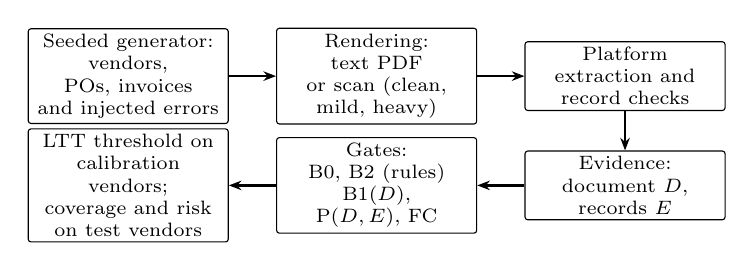
\begin{tikzpicture}[
  box/.style={draw, rounded corners=1pt, align=center, font=\scriptsize,
              minimum height=8mm, text width=24mm, inner sep=2pt},
  arr/.style={-{Stealth[length=1.6mm]}, thick},
  node distance=5mm and 6mm]
\node[box] (gen) {Seeded generator:\\vendors, POs, invoices\\and injected errors};
\node[box, right=of gen] (ren) {Rendering: text PDF\\or scan (clean,\\mild, heavy)};
\node[box, right=of ren] (ext) {Platform\\extraction and\\record checks};
\node[box, below=of ext] (feat) {Evidence:\\document $D$,\\records $E$};
\node[box, left=of feat] (gate) {Gates:\\B0, B2 (rules)\\B1($D$), P($D,E$), FC};
\node[box, left=of gate] (eval) {LTT threshold on\\calibration vendors;\\coverage and risk\\on test vendors};
\draw[arr] (gen) -- (ren);
\draw[arr] (ren) -- (ext);
\draw[arr] (ext) -- (feat);
\draw[arr] (feat) -- (gate);
\draw[arr] (gate) -- (eval);
\end{tikzpicture}}
\caption{Evaluation pipeline. Training, calibration and test sets contain
different vendors; the procedure is repeated over 20 random splits.}
\label{fig:pipeline}
\end{figure}

\subsection{Deployed Rule and Extraction}\label{sec:deployed}
In the study, text PDFs are read with a text-layer parser and scans with
PaddleOCR using the platform's settings and line parsing \cite{cui2025paddleocr};
a machine-learning classifier assigns the document type and regular expressions
extract the fields. (The live pipeline also routes scanned PDFs through
Docling \cite{auer2024docling} and cross-checks fields with LayoutLMv3; neither
path is part of this study.) Each field $f$ has a confidence $c_f\in[0,1]$,
discounted by the quality $q\in[0,1]$ of the text it was read from. The
document score is a weighted mean:
\begin{equation}
s_f = c_f\,q,\quad
S=\frac{\sum_{f\in F} w_f\, s_f}{\sum_{f\in F} w_f},\quad
\text{review if } S<\theta=0.8,
\label{eq:conf}
\end{equation}
with $w_f$ = 0.30 (total), 0.20 (vendor name), 0.15 (classification), 0.15
(document number), 0.10 (date) and 0.10 (line items, left out when none are
found). The deployed rule also forces review when the
vendor name is missing or resembles but does not match a known vendor, when the
document is not recognized as an invoice, when the PO match fails, when a
duplicate is found, or when bank details differ from the master. Confidence and
these flags together form baseline \sysB.

\subsection{Synthetic Procure-to-Pay World}
A seeded generator builds a vendor master of 100 vendors, each with a Goods and
Services Tax Identification Number (GSTIN), bank details and a currency (15\% of
vendors invoice in US dollars, the rest in Indian rupees, INR). Invoice volume
follows a Zipf-like weight $1/(1+i)^{0.8}$ over vendors, so a few vendors send
most invoices; the largest sends 350 of the 3,000. The generator then issues
1,649 POs and 3,000 invoices against them. Each invoice carries at most one
injected business error of eight types, listed with their counts in
Table~\ref{tab:data}. A resubmitted duplicate copies an earlier invoice of the
same vendor, moves its date by one to three days, and always takes the vendor's
next invoice number. Invoices are rendered as text PDFs or as clean, mildly
degraded or heavily degraded scans. Ground truth is known by construction.

\begin{table}[t]
\caption{Synthetic Benchmark (Generator 1.0, Seed 7)}
\begin{center}
\begin{tabular}{|l|r|}
\hline
\textbf{Item} & \textbf{Value} \\
\hline
Vendors / purchase orders / invoices & 100 / 1,649 / 3,000 \\
Invoices with an injected error & 895 (29.8\%) \\
\quad duplicate (renumbered resubmission) & 147 \\
\quad unit price above the PO & 145 \\
\quad changed bank details & 117 \\
\quad quantity above the PO's remainder & 109 \\
\quad total not equal to subtotal plus tax & 109 \\
\quad look-alike vendor name & 95 \\
\quad another vendor's PO cited & 88 \\
\quad wrong or invalid GSTIN & 85 \\
Fields read correctly & 84.3\% \\
Correct invoices ($Y=1$) & 59.9\% \\
\hline
\multicolumn{2}{|l|}{\textit{Share / fields read correctly / correct invoices}$^{\mathrm{a}}$} \\
\quad text PDF & 55.1 / 100 / 72.3 \\
\quad clean scan & 25.5 / 91.2 / 63.0 \\
\quad mild scan & 11.5 / 51.7 / 34.7 \\
\quad heavy scan & 7.9 / 0.0 / 0.0 \\
\hline
\multicolumn{2}{l}{$^{\mathrm{a}}$All three values in percent.}
\end{tabular}
\label{tab:data}
\end{center}
\end{table}

So 40.1\% of invoices are incorrect: 29.8 points from injected errors and 10.3
points from misread fields alone. Heavy scans are never read correctly, which
makes them easy to reject; the mild scans are where reading errors are hard to
spot.

\subsection{Record Checks}
The checks reuse the platform's rules. Vendor matching compares the normalized
name with the master by fuzzy token ratio; a score of 88 or more is a match and
70 to 87 a look-alike. The three-way match compares the invoice's lines with the
vendor's open POs and holds the invoice when a unit price or the remaining
balance is exceeded by more than 1\%. Bank details, GSTIN and currency are
compared with the master. Two invoices $i,j$ of the same vendor are duplicates
when
\begin{equation}
|a_i-a_j|\le 0.02\,a_j \ \wedge\ |d_i-d_j|\le 7\ \text{days}\ \wedge\
\mathrm{sim}(n_i,n_j)\ge 0.85,
\label{eq:dup}
\end{equation}
where $a$ is the amount, $d$ the date, $n$ the invoice number and $\mathrm{sim}$
a string-similarity ratio. All three limits are configurable business
rules. The exploratory check of Section~\ref{sec:posthoc}
drops the last condition, which equals setting that rule to zero. The checks add
about 1~ms per invoice.

\subsection{Gate Systems}\label{sec:systems}
We compare five systems:
\begin{itemize}
\item \sysB: the deployed rule of Section~\ref{sec:deployed}.
\item \sysBtwo: accept when every record check passes (vendor matched and not a
look-alike, PO matched, no duplicate, and bank details, GSTIN and currency agree
with the master where present). It ignores extraction confidence.
\item \sysBone: a probability model of $\Pr[Y=1]$ on 19 document features,
thresholded with LTT.
\item \sysP: the same on the document features plus 16 record features (vendor,
PO, duplicate, bank, GSTIN, currency, vendor history).
\item \sysFC: one LTT gate per payment-critical component (vendor, total,
currency, number, business error), each at $\alpha/5$ so that a union bound gives
document-level risk $\alpha$; an invoice is accepted when all five accept (RQ3).
\end{itemize}
The probability model is either a standardized logistic regression or histogram
gradient boosting (scikit-learn \cite{pedregosa2011}; 300 iterations, learning
rate 0.05, 15 leaves, L2 penalty 1.0). \sysFC{} uses logistic regression.
Fig.~\ref{fig:gate} shows how a learned gate decides for one invoice: the
probability model scores the evidence, and the invoice is posted only if the
score clears the threshold chosen by LTT on the calibration vendors.

\begin{figure}[t]
\centering
\resizebox{\columnwidth}{!}{%
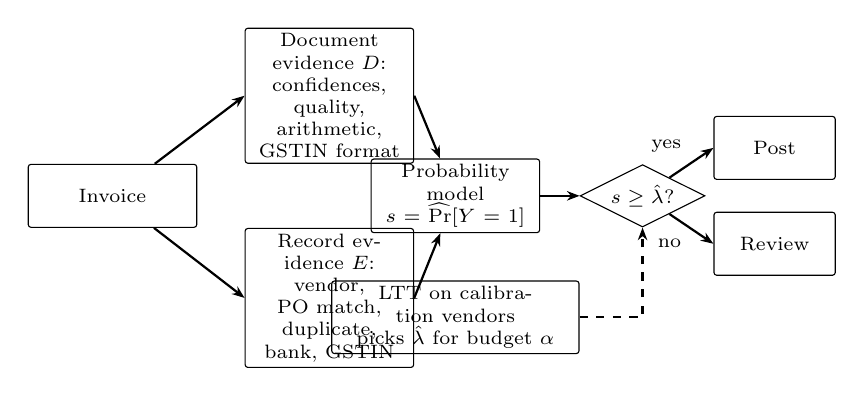
\begin{tikzpicture}[
  box/.style={draw, rounded corners=1pt, align=center, font=\scriptsize,
              minimum height=8mm, text width=20mm, inner sep=2pt},
  dec/.style={draw, diamond, aspect=2, align=center, font=\scriptsize, inner sep=1pt},
  arr/.style={-{Stealth[length=1.6mm]}, thick},
  node distance=4mm and 5mm]
\node[box] (inv) {Invoice};
\node[box, above right=0mm and 6mm of inv] (d) {Document evidence $D$:\\confidences, quality,\\arithmetic, GSTIN format};
\node[box, below right=0mm and 6mm of inv] (e) {Record evidence $E$:\\vendor, PO match,\\duplicate, bank, GSTIN};
\node[box, right=22mm of inv] (m) {Probability\\model\\$s=\widehat{\Pr}[Y=1]$};
\node[dec, right=of m] (t) {$s\ge\hat\lambda$?};
\node[box, above right=0mm and 5mm of t, text width=14mm] (post) {Post};
\node[box, below right=0mm and 5mm of t, text width=14mm] (rev) {Review};
\node[box, below=6mm of m, text width=30mm] (ltt) {LTT on calibration vendors\\picks $\hat\lambda$ for budget $\alpha$};
\draw[arr] (inv) -- (d.west);
\draw[arr] (inv) -- (e.west);
\draw[arr] (d.east) -- (m);
\draw[arr] (e.east) -- (m);
\draw[arr] (m) -- (t);
\draw[arr] (t) -- node[font=\scriptsize, above left]{yes} (post.west);
\draw[arr] (t) -- node[font=\scriptsize, below left]{no} (rev.west);
\draw[arr, dashed] (ltt) -| (t);
\end{tikzpicture}}
\caption{Decision of a learned gate (\sysP) for one invoice. \sysBone{} uses only
the document evidence.}
\label{fig:gate}
\end{figure}

% ---------------------------------------------------------------------
\section{Experimental Setup}\label{sec:setup}
Each of 20 random splits assigns vendors 50/25/25 to training, calibration and
test, so test vendors are never seen before. The model is fitted on training
vendors. Candidate thresholds come from training-score quantiles at 40 coverage
levels, starting where a rejection is possible, as set by \eqref{eq:floor}; LTT
then picks one on the calibration vendors with $\delta=0.1$. The plan fixed
error budgets of 1\%, 2\% and 5\%; we added 10\% after nothing passed at 5\%,
and use it only for the ablation and the stale-records test.

For each system we report means over splits of coverage \eqref{eq:cov} and risk
\eqref{eq:risk} on the test vendors, and the \emph{violation rate}, the share of
splits with test risk above $\alpha$, which should be at most $\delta$. For the
learned gates we also report the area under the receiver operating
characteristic curve (AUROC) and the area under the risk--coverage curve (AURC).
We give the value in INR of wrongly accepted invoices. Coverage differences
between systems get a paired percentile bootstrap 95\% confidence interval (CI)
over splits. A gate that accepts nothing has its risk shown as a dash.

For RQ4 we make a share of the records stale (0 to 40\%): those vendors' bank
details change and their GSTIN goes missing, and the same share of POs is never
entered. Everything runs from one script that writes all figures to a results
file, with the generator version, seed and code commit recorded
\todo{add repository link or data-availability statement}.

% ---------------------------------------------------------------------
\section{Results and Discussion}\label{sec:results}
Table~\ref{tab:main} gives the main results, and Fig.~\ref{fig:coverage} plots
coverage across all four budgets and risk against coverage at the 5\% budget.

\begin{table}[t]
\caption{Review Gates on 3,000 Synthetic Invoices, Means over 20 Vendor-Disjoint Splits}
\begin{center}
\setlength{\tabcolsep}{2.5pt}
\resizebox{\columnwidth}{!}{%
\begin{tabular}{|l|c|c|c|c|c|c|}
\hline
\textbf{System} & \multicolumn{2}{c|}{\textbf{$\alpha=2\%$}} & \multicolumn{2}{c|}{\textbf{$\alpha=5\%$}} & \textbf{AUROC} & \textbf{AURC} \\
\cline{2-5}
 & \textbf{\textit{Cov.}} & \textbf{\textit{Risk}} & \textbf{\textit{Cov.}} & \textbf{\textit{Risk}} & & \\
\hline
\sysB: deployed rule$^{\mathrm{a}}$ & 41.2\% & 6.8\% & 41.2\% & 6.8\% & -- & -- \\
\sysBtwo: all record checks$^{\mathrm{a}}$ & 58.9\% & 12.8\% & 58.9\% & 12.8\% & -- & -- \\
\sysBone: document only$^{\mathrm{b}}$ & 0.0\% & -- & 0.0\% & -- & 0.724 & 0.269 \\
\sysP: document and records$^{\mathrm{b}}$ & 0.0\% & -- & 1.7\% & 0.2\% & 0.947 & 0.124 \\
\sysFC: per component & 0.0\% & -- & 0.0\% & -- & -- & -- \\
\hline
\sysPdup$^{\mathrm{b,c}}$ & 12.1\% & 0.3\% & 35.4\% & 2.3\% & 0.971 & 0.106 \\
\hline
\multicolumn{7}{p{1.2\columnwidth}}{\footnotesize Cov.: share of test invoices
accepted without review. Risk: share of accepted invoices that are wrong.
At $\alpha=1\%$ every gate accepts nothing.} \\
\multicolumn{7}{p{1.2\columnwidth}}{\footnotesize $^{\mathrm{a}}$Fixed rules:
they violate the 2\% budget in all splits and the 5\% budget in 90\% (\sysB)
and 100\% (\sysBtwo) of splits.} \\
\multicolumn{7}{p{1.2\columnwidth}}{\footnotesize $^{\mathrm{b}}$Gradient
boosting. With logistic regression the AUROCs are 0.741, 0.938 and 0.954,
\sysP{} accepts nothing, and \sysPdup{} covers 2.0\% and 7.9\%.} \\
\multicolumn{7}{p{1.2\columnwidth}}{\footnotesize $^{\mathrm{c}}$Defined post
hoc (Section~\ref{sec:posthoc}); violation rate 5\% at $\alpha=2\%$ and 10\% at
$\alpha=5\%$.}
\end{tabular}}
\label{tab:main}
\end{center}
\end{table}

\begin{figure*}[t]
\centering
\begin{subfigure}[t]{0.48\textwidth}
\centering
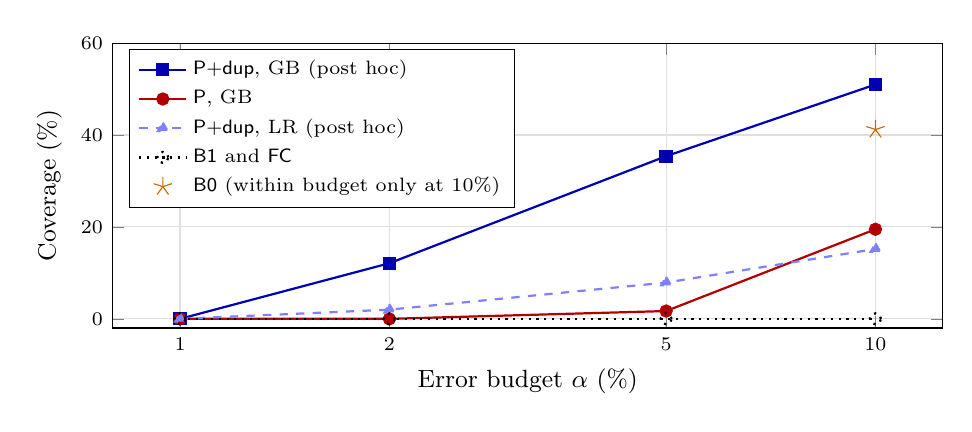
\begin{tikzpicture}
\begin{axis}[
  width=\linewidth, height=5.2cm,
  xmode=log, xmin=0.8, xmax=12.5,
  xtick={1,2,5,10}, xticklabels={1,2,5,10},
  xlabel={Error budget $\alpha$ (\%)}, ylabel={Coverage (\%)},
  ymin=-2, ymax=60, grid=major, grid style={gray!25},
  legend style={font=\scriptsize, at={(0.02,0.98)}, anchor=north west, cells={anchor=west}},
  tick label style={font=\scriptsize}, label style={font=\small}]
\addplot[thick, mark=square*, color=blue!70!black] coordinates {(1,0) (2,12.1) (5,35.4) (10,51.0)};
\addlegendentry{\sysPdup, GB (post hoc)}
\addplot[thick, mark=*, color=red!70!black] coordinates {(1,0) (2,0) (5,1.7) (10,19.5)};
\addlegendentry{\sysP, GB}
\addplot[thick, dashed, mark=triangle*, color=blue!50] coordinates {(1,0) (2,2.0) (5,7.9) (10,15.2)};
\addlegendentry{\sysPdup, LR (post hoc)}
\addplot[thick, dotted, mark=o, color=black] coordinates {(1,0) (2,0) (5,0) (10,0)};
\addlegendentry{\sysBone{} and \sysFC}
\addplot[only marks, mark=star, mark size=3.5pt, color=orange!80!black] coordinates {(10,41.2)};
\addlegendentry{\sysB{} (within budget only at 10\%)}
\end{axis}
\end{tikzpicture}
\caption{Coverage that each system achieves while meeting the budget.}
\label{fig:cov-alpha}
\end{subfigure}\hfill
\begin{subfigure}[t]{0.48\textwidth}
\centering
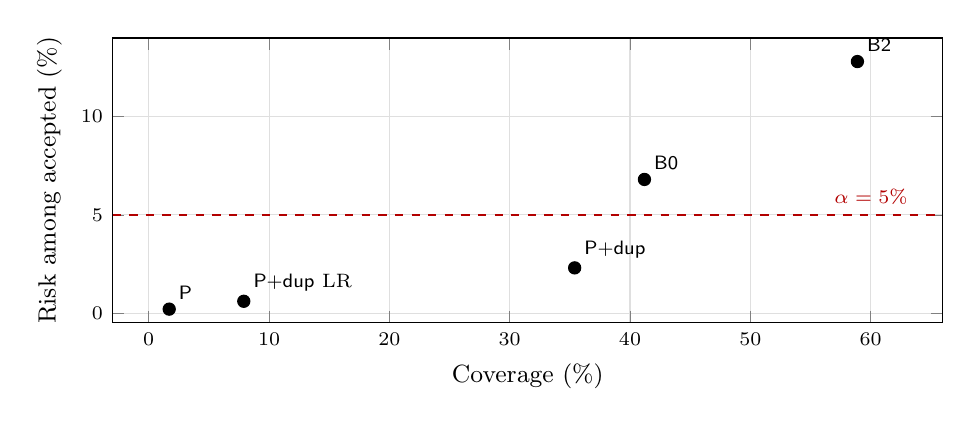
\begin{tikzpicture}
\begin{axis}[
  width=\linewidth, height=5.2cm,
  xlabel={Coverage (\%)}, ylabel={Risk among accepted (\%)},
  xmin=-3, xmax=66, ymin=-0.5, ymax=14, grid=major, grid style={gray!25},
  tick label style={font=\scriptsize}, label style={font=\small},
  nodes near coords, point meta=explicit symbolic,
  every node near coord/.append style={font=\scriptsize, anchor=south west}]
\addplot[only marks, mark=*, mark size=2.2pt, color=black] coordinates {
  (41.2,6.8)[\sysB] (58.9,12.8)[\sysBtwo] (1.7,0.2)[\sysP] (35.4,2.3)[\sysPdup] (7.9,0.6)[\sysPdup{} LR]};
\draw[thick, dashed, red!70!black] (axis cs:-3,5) -- (axis cs:66,5)
  node[pos=0.97, above left, font=\scriptsize] {$\alpha=5\%$};
\end{axis}
\end{tikzpicture}
\caption{Risk against coverage at $\alpha=5\%$; points above the line break the budget.}
\label{fig:risk-cov}
\end{subfigure}
\caption{Coverage and risk of the review gates (means over 20 splits; GB:
gradient boosting, LR: logistic regression). The fixed rules accept many
invoices but break the 2\% and 5\% budgets; the pre-specified learned gates meet
the budgets by accepting almost nothing below 10\%.}
\label{fig:coverage}
\end{figure*}

\subsection{Error Rate of the Deployed Rule}\label{sec:rq1}
\sysB{} accepts 41.2\% of invoices ($\pm$1.2 points across splits), and 6.8\%
of those are wrong, so about 2.8\% of all invoices would be paid in error. The
wrongly accepted invoices are worth INR 15.5 million (154.6 lakh) per test set
on average. Trusting the record checks alone (\sysBtwo) covers more, 58.9\%, at
almost twice the risk (12.8\%, INR 40.1 million). \sysB{} already raises most
of these checks as review flags, so its errors are invoices that pass the flags
as they are configured, not only errors that confidence cannot see. Neither rule
meets a 2\% or 5\% budget (Fig.~\ref{fig:risk-cov}). \sysB{} does meet a 10\%
budget in every split (its highest split risk is 8.6\%). A breakdown of the
accepted errors of \sysB{} by injected type would show which checks let them
through \todo{run the failure breakdown for \sysB{} and \sysBtwo}.

\subsection{Value of Record Evidence}\label{sec:rq2}
Record evidence raises AUROC from 0.724 to 0.947 with gradient boosting and from
0.741 to 0.938 with logistic regression, and halves AURC (0.269 to 0.124). The
PO match carries most of this (Fig.~\ref{fig:ablation}). Removing it lowers the
logistic AUROC from 0.938 to 0.831; removing bank details, the duplicate check
or the GSTIN check gives 0.897, 0.919 and 0.921, while vendor matching, currency
and history change it by at most 0.002. The three-way match runs only for a
matched vendor, so the PO features already carry most of what vendor matching
adds.

Better ranking did not become coverage at the planned budgets. \sysP{}
certifies nothing at 1\% and 2\% and 1.7\% at 5\% (risk 0.2\%, no violations);
\sysBone{} certifies nothing. The paired gain of \sysP{} over \sysBone{} is
$+0.0$ points at $\alpha=2\%$ and $+1.7$ points (95\% CI $[0.0,5.1]$) at 5\%,
so H1 is not supported. The gain appears only at the looser 10\% budget, which
was not in the plan: \sysP{} then covers 19.5\% at 2.7\% risk and 5\% violations,
a gain of $+19.5$ points (CI $[8.4,31.6]$) over \sysBone{}
(Fig.~\ref{fig:cov-alpha}).

\begin{figure*}[t]
\centering
\begin{subfigure}[t]{0.48\textwidth}
\centering
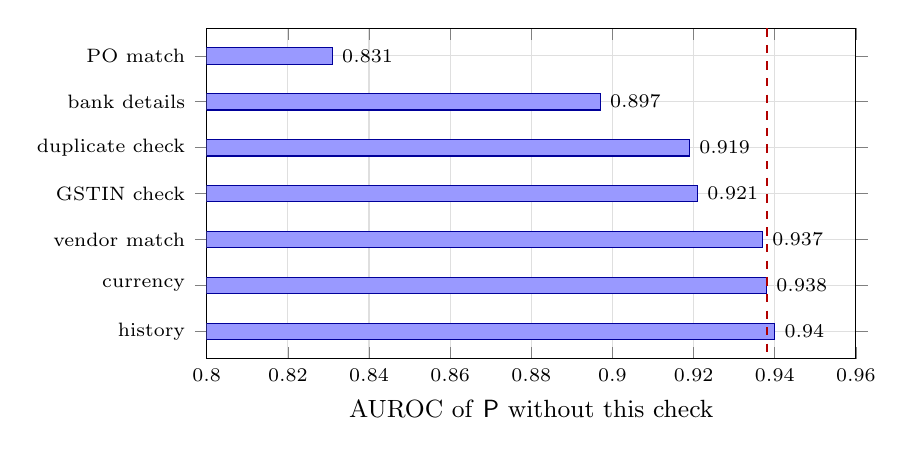
\begin{tikzpicture}
\begin{axis}[
  width=0.68\linewidth, height=4.2cm, scale only axis,
  xbar, bar width=6pt, xmin=0.80, xmax=0.96,
  xlabel={AUROC of \sysP{} without this check},
  ytick={1,...,7}, y dir=reverse, ymin=0.4, ymax=7.6,
  yticklabels={PO match,bank details,duplicate check,GSTIN check,vendor match,currency,history},
  tick label style={font=\scriptsize}, label style={font=\small},
  nodes near coords, nodes near coords style={font=\scriptsize},
  every node near coord/.append style={/pgf/number format/.cd, fixed, precision=3},
  grid=major, grid style={gray!25}]
\addplot[fill=blue!40, draw=blue!60!black] coordinates {
  (0.831,1) (0.897,2) (0.919,3) (0.921,4) (0.937,5) (0.938,6) (0.940,7)};
\draw[thick, dashed, red!70!black] (axis cs:0.938,0.4) -- (axis cs:0.938,7.6);
\end{axis}
\end{tikzpicture}
\caption{Ablation: AUROC with one group of record checks removed. Dashed line:
all checks (0.938).}
\label{fig:ablation-bars}
\end{subfigure}\hfill
\begin{subfigure}[t]{0.48\textwidth}
\centering
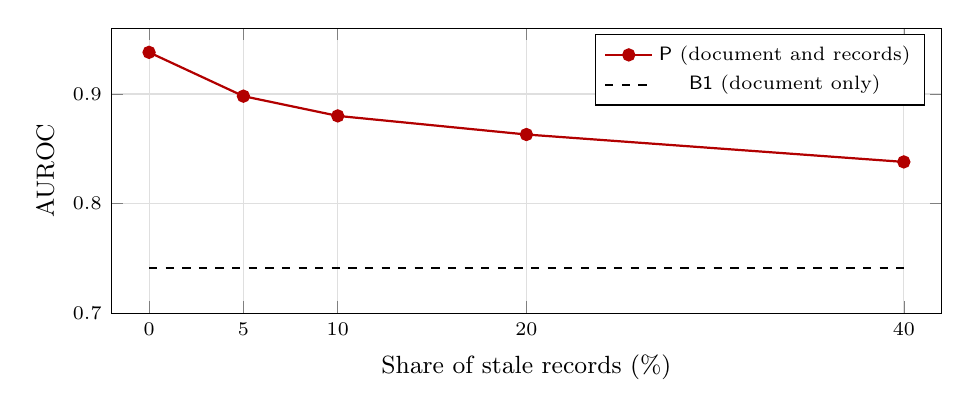
\begin{tikzpicture}
\begin{axis}[
  width=\linewidth, height=5.2cm,
  xlabel={Share of stale records (\%)}, ylabel={AUROC},
  xmin=-2, xmax=42, ymin=0.70, ymax=0.96,
  xtick={0,5,10,20,40},
  grid=major, grid style={gray!25},
  legend style={font=\scriptsize, at={(0.98,0.98)}, anchor=north east},
  tick label style={font=\scriptsize}, label style={font=\small},
  yticklabel style={/pgf/number format/.cd, fixed, precision=2}]
\addplot[thick, mark=*, color=red!70!black] coordinates {(0,0.938) (5,0.898) (10,0.880) (20,0.863) (40,0.838)};
\addlegendentry{\sysP{} (document and records)}
\addplot[thick, dashed, color=black] coordinates {(0,0.741) (40,0.741)};
\addlegendentry{\sysBone{} (document only)}
\end{axis}
\end{tikzpicture}
\caption{Stale records: AUROC as bank details, GSTINs and POs go out of date.}
\label{fig:stale}
\end{subfigure}
\caption{Where the ranking signal comes from and how it decays (logistic
regression, means over 20 splits). The PO match carries most of the signal;
with 40\% of the records stale, \sysP{} still ranks better than \sysBone.}
\label{fig:ablation}
\end{figure*}

\subsection{Why the Gates Certify Little}\label{sec:why}
Among the invoices \sysP{} ranks highest, about 5\% are still wrong. By
\eqref{eq:floor}, a 2\% budget needs at least 114 accepted calibration invoices
with almost no errors (Table~\ref{tab:floor}), and an error rate of 5\% at the
top of the ranking makes that impossible; LTT therefore accepts nothing.
Inspecting these invoices showed that most were renumbered resubmissions. The
duplicate rule \eqref{eq:dup} needs the two invoice numbers to be at least 85\%
similar, which a new number often is not, and the PO still has quantity left, so
the three-way match passes too. The rest were mostly overbilled invoices whose
scanned line items were misread, which hides the excess from the three-way
match. The limit lies in one check, not in the probability model.

\subsection{Exploratory Number-Independent Duplicate Check}\label{sec:posthoc}
Adding a feature for the duplicate check without its number condition gives
\sysPdup. With gradient boosting it certifies 12.1\% of invoices at
$\alpha=2\%$ (risk 0.3\%) and 35.4\% at 5\% (risk 2.3\%), with AUROC 0.971 and
violation rates of 5\% and 10\%. With 20 splits, a 10\% violation rate has a
standard error of about 0.07 ($\sqrt{0.1\cdot0.9/20}$), which is consistent
with $\delta=0.1$ but cannot confirm it. At 10\% the violation rate rises to
20\%, above $\delta$. The gate was defined after we saw the diagnosis, on the
same seed, and the generator gives every duplicate a new number. It is a
hypothesis for a new seed and for external data, not a result.

Table~\ref{tab:failures} lists the largest groups of invoices that \sysPdup{}
still accepts wrongly at $\alpha=10\%$. Arithmetic errors and overbilled prices
on clean scans lead, followed by correct invoices whose total or number was
misread on a scan. Renumbered duplicates still appear, mostly on clean scans,
where the amount or date was read differently from the original.

\begin{table}[t]
\caption{Largest Groups of Wrongly Accepted Invoices, \sysPdup{} with Gradient
Boosting at \boldmath$\alpha=10\%$, Summed over 20 Splits}
\begin{center}
\begin{tabular}{|l|l|l|r|}
\hline
\textbf{Injected error} & \textbf{Rendering} & \textbf{Misread field} & \textbf{Count} \\
\hline
total $\neq$ subtotal plus tax & clean scan & none & 99 \\
unit price above PO & clean scan & none & 62 \\
none & mild scan & total & 54 \\
none & clean scan & number & 43 \\
quantity above PO & clean scan & none & 37 \\
duplicate & clean scan & none & 36 \\
\hline
\end{tabular}
\label{tab:failures}
\end{center}
\end{table}

\subsection{Per-Component Gates and Stale Records}\label{sec:rq34}
\sysFC{} accepts nothing at any budget. Each component gate runs at $\alpha/5$,
which raises the floor to 575 accepted calibration invoices at a 2\% budget and
230 at 5\% (Table~\ref{tab:floor}), each with almost no errors for that
component. The study therefore says nothing for or against document-level
control yet (RQ3).

With stale records (RQ4), the AUROC of \sysP{} falls steadily, from 0.938 to
0.898, 0.880, 0.863 and 0.838 as 5, 10, 20 and 40\% of the records go stale
(logistic, $\alpha=10\%$; Fig.~\ref{fig:stale}). It stays above the
document-only 0.741 at every level. Coverage is near zero at all levels, so the
effect of stale records on coverage remains unmeasured.

% ---------------------------------------------------------------------
\section{Limitations}\label{sec:limits}
The invoices, records and error rates come from one seeded generator, and no
real or public invoice data were used; absolute coverage and risk will not
transfer to another organization. The generator also decides how detectable each
error is. Every injected duplicate carries a new number, so the gain from the
number-independent check partly reflects that design choice. The planned
external-validity run on public invoices with derived records has not been done.
The \sysPdup{} gate was chosen after inspecting results and has been run on one
seed only.

Vendors are assigned to calibration and test at random, but invoices of one
vendor are not independent, and the binomial test \eqref{eq:pval} treats them as
if they were. With one vendor sending 350 of 3,000 invoices, the effective
calibration size is smaller than the count and varies across splits, which may
explain violation rates above $\delta$. No correction for this, such as
cluster-aware bounds or weighted calibration \cite{tibshirani2019}, was applied.

The study covers 100 vendors, so each calibration set holds 25 of them and the
bounds are wide; it also uses a single $\delta$. Reviewers are treated as free
and always right, unlike in learning-to-defer formulations \cite{mozannar2020}.
Results depend on one extraction stack, and the Docling and LayoutLMv3 paths of
the live pipeline were not exercised. Finally, the literature search ran in
October 2026 through web search and Crossref, not through subscription indexes,
and this area moved quickly in 2026.

% ---------------------------------------------------------------------
\section{Conclusion}\label{sec:conclusion}
On a synthetic P2P benchmark, a hand-set confidence rule accepted 41.2\% of
invoices with 6.8\% of them wrong, above both budgets we planned to certify.
Record evidence improved the ranking of invoices substantially, mostly through
the PO match, but no pre-specified risk-controlled gate certified more than
1.7\% of invoices at budgets of 5\% or less, and the pre-registered gain was not
found. The bottleneck was one rule: resubmitted invoices with a new number pass
the duplicate check. A check that ignores the number certified 12.1\% and 35.4\%
at the 2\% and 5\% budgets, but it was found by looking at the results.

Next we will repeat the study on new generator seeds and on public invoices
(DocILE or FATURA) with derived records, vary the share of renumbered
resubmissions, use cluster-aware bounds for vendor-grouped data, give \sysFC{}
enough calibration data to answer RQ3, and model reviewer error and cost.

% ---------------------------------------------------------------------
% Reference order = order of first citation in the text. Template rules:
% list all authors unless there are six or more; titles in sentence case;
% unpublished work marked "unpublished".
\begin{thebibliography}{00}

% VERIFIED-D1
\bibitem{elyaniv2010}
R. El-Yaniv and Y. Wiener, ``On the foundations of noise-free selective
classification,'' \emph{J. Mach. Learn. Res.}, vol. 11, pp. 1605--1641, 2010.

% VERIFIED-D1 (arXiv:1705.08500)
\bibitem{geifman2017}
Y. Geifman and R. El-Yaniv, ``Selective classification for deep neural
networks,'' in \emph{Advances in Neural Information Processing Systems 30}, 2017,
pp. 4878--4887.

% VERIFIED-GA (ICDAR 2019 proceedings)
\bibitem{huang2019sroie}
Z. Huang, K. Chen, J. He, X. Bai, D. Karatzas, S. Lu, and C. V. Jawahar,
``ICDAR2019 competition on scanned receipt OCR and information extraction,''
in \emph{Proc. Int. Conf. Document Analysis and Recognition (ICDAR)}, 2019,
pp. 1516--1520, doi:10.1109/ICDAR.2019.00244.

% VERIFIED-GA
\bibitem{huang2022layoutlmv3}
Y. Huang, T. Lv, L. Cui, Y. Lu, and F. Wei, ``LayoutLMv3: Pre-training for
document AI with unified text and image masking,'' in \emph{Proc. 30th ACM Int.
Conf. Multimedia}, 2022, pp. 4083--4091, doi:10.1145/3503161.3548112.

% VERIFIED-GA (vol. 19)
\bibitem{angelopoulos2025ltt}
A. N. Angelopoulos, S. Bates, E. J. Cand\`es, M. I. Jordan, and L. Lei, ``Learn
then test: Calibrating predictive algorithms to achieve risk control,''
\emph{Ann. Appl. Statist.}, vol. 19, pp. 1641--1662, 2025,
doi:10.1214/24-AOAS1998.

% VERIFIED-GA (preprint, more than six authors; check for a published
% version before submission)
\bibitem{jin2026plv}
Y. Jin, Y. Wang, Y. Han, C. Y. S. Kwan, W. Song \emph{et al.}, ``Perception,
layout, and validation: Calibrated confidence for reliable straight-through
processing of financial documents,'' arXiv:2609.20110, 2026.

% VERIFIED-GA
\bibitem{rombach2026}
A. Rombach and N. Mehdiyev, ``Beyond accuracy: Understanding model confidence in
key information extraction with conformal prediction,'' \emph{Int. J. Document
Analysis and Recognition}, vol. 29, no. 2, pp. 551--563, 2026,
doi:10.1007/s10032-026-00572-y.

% VERIFIED-GA (product documentation, accessed 16 Oct 2026)
\bibitem{rossum2026}
Rossum, ``Automation rules overview'' and ``Master data hub,'' product
documentation. [Online]. Available:
\url{https://knowledge-base.rossum.ai/docs/automation-rules-overview}, accessed
Oct. 16, 2026.

% VERIFIED-GA (product documentation, accessed 16 Oct 2026)
\bibitem{sapariba2026}
SAP, ``Understanding invoice reconciliation,'' SAP Ariba procurement overview,
SAP Learning. [Online]. Available:
\url{https://learning.sap.com/courses/sap-ariba-procurement-overview-1/understanding-invoice-reconciliation-1},
accessed Oct. 16, 2026.

% VERIFIED-GA (ICLR 2024)
\bibitem{angelopoulos2024crc}
A. N. Angelopoulos, S. Bates, A. Fisch, L. Lei, and T. Schuster, ``Conformal risk
control,'' in \emph{Proc. Int. Conf. Learning Representations (ICLR)}, 2024.

% VERIFIED-D1 (arXiv:1711.06664)
\bibitem{madras2018}
D. Madras, T. Pitassi, and R. Zemel, ``Predict responsibly: Improving fairness
and accuracy by learning to defer,'' in \emph{Advances in Neural Information
Processing Systems 31}, 2018, pp. 6147--6157.

% VERIFIED-GA (PMLR 119)
\bibitem{mozannar2020}
H. Mozannar and D. Sontag, ``Consistent estimators for learning to defer to an
expert,'' in \emph{Proc. 37th Int. Conf. Machine Learning}, PMLR vol. 119, 2020,
pp. 7076--7087.

% VERIFIED-D1
\bibitem{guo2017}
C. Guo, G. Pleiss, Y. Sun, and K. Q. Weinberger, ``On calibration of modern
neural networks,'' in \emph{Proc. 34th Int. Conf. Machine Learning}, PMLR vol.
70, 2017, pp. 1321--1330.

% VERIFIED-D1 (arXiv:1904.06019)
\bibitem{tibshirani2019}
R. J. Tibshirani, R. F. Barber, E. J. Cand\`es, and A. Ramdas, ``Conformal
prediction under covariate shift,'' in \emph{Advances in Neural Information
Processing Systems 32}, 2019, pp. 2530--2540.

% CARRIED from project report (more than six authors)
\bibitem{cui2025paddleocr}
C. Cui \emph{et al.}, ``PaddleOCR 3.0 technical report,'' arXiv:2507.05595, 2025.

% VERIFIED-GA (more than six authors)
\bibitem{auer2024docling}
C. Auer, M. Lysak, A. Nassar, M. Dolfi, N. Livathinos \emph{et al.}, ``Docling
technical report,'' arXiv:2408.09869, 2024.

% VERIFIED-GA (arXiv:2302.05658; proceedings DOI not verified; 11 authors)
\bibitem{simsa2023docile}
\v{S}. \v{S}imsa, M. \v{S}ulc, M. U\v{r}i\v{c}\'a\v{r}, Y. Patel, A. Hamdi
\emph{et al.}, ``DocILE benchmark for document information localization and
extraction,'' in \emph{Proc. Int. Conf. Document Analysis and Recognition
(ICDAR)}, 2023.

% VERIFIED-GA (preprint; dataset on Zenodo)
\bibitem{limam2023fatura}
M. Limam, M. Dhiaf, and Y. Kessentini, ``FATURA: A multi-layout invoice image
dataset for document analysis and understanding,'' arXiv:2311.11856, 2023.

% VERIFIED-GA
\bibitem{krieger2023}
F. Krieger, P. Drews, and B. Funk, ``Automated invoice processing: Machine
learning-based information extraction for long tail suppliers,''
\emph{Intelligent Systems with Applications}, vol. 20, art. 200285, 2023,
doi:10.1016/j.iswa.2023.200285.

% VERIFIED-GA (preprint; KDD 2021 Document Intelligence workshop)
\bibitem{nguyen2022hycedis}
B.-S. Nguyen, Q.-B. Tran, T.-A. Nguyen Dang, D. Nguyen, and H. Le, ``HYCEDIS:
HYbrid confidence engine for deep document intelligence system,''
arXiv:2206.02628, 2022.

% VERIFIED-GA (preprint; nine authors)
\bibitem{roy2026confbench}
P. Roy, S. Martin, M. Rostami, S. Romo, R. Xue \emph{et al.}, ``Can you trust the
confidence? ConfBench for vision-language models on document extraction,''
arXiv:2608.01792, 2026.

% VERIFIED-GA
\bibitem{guida2023}
M. Guida, F. Caniato, A. Moretto, and S. Ronchi, ``The role of artificial
intelligence in the procurement process: State of the art and research agenda,''
\emph{J. Purchasing and Supply Management}, vol. 29, art. 100823, 2023,
doi:10.1016/j.pursup.2023.100823.

% VERIFIED-GA
\bibitem{spreitzenbarth2024}
J. M. Spreitzenbarth, C. Bode, and H. Stuckenschmidt, ``Artificial intelligence
and machine learning in purchasing and supply management: A mixed-methods review
of the state-of-the-art in literature and practice,'' \emph{J. Purchasing and
Supply Management}, vol. 30, art. 100896, 2024,
doi:10.1016/j.pursup.2024.100896.

% CARRIED from project report (more than six authors)
\bibitem{pedregosa2011}
F. Pedregosa \emph{et al.}, ``Scikit-learn: Machine learning in Python,''
\emph{J. Mach. Learn. Res.}, vol. 12, pp. 2825--2830, 2011.

\end{thebibliography}

\end{document}
